\documentclass[tikz,border=10pt]{standalone}
\usepackage{tikz}
\usetikzlibrary{positioning}

% Global styles for nodes and paths
\tikzset{
  every node/.style={text=black, draw=black, font=\Large, line width=0.5mm},
  every path/.style={draw=black, line width=0.5mm}
}

\begin{document}
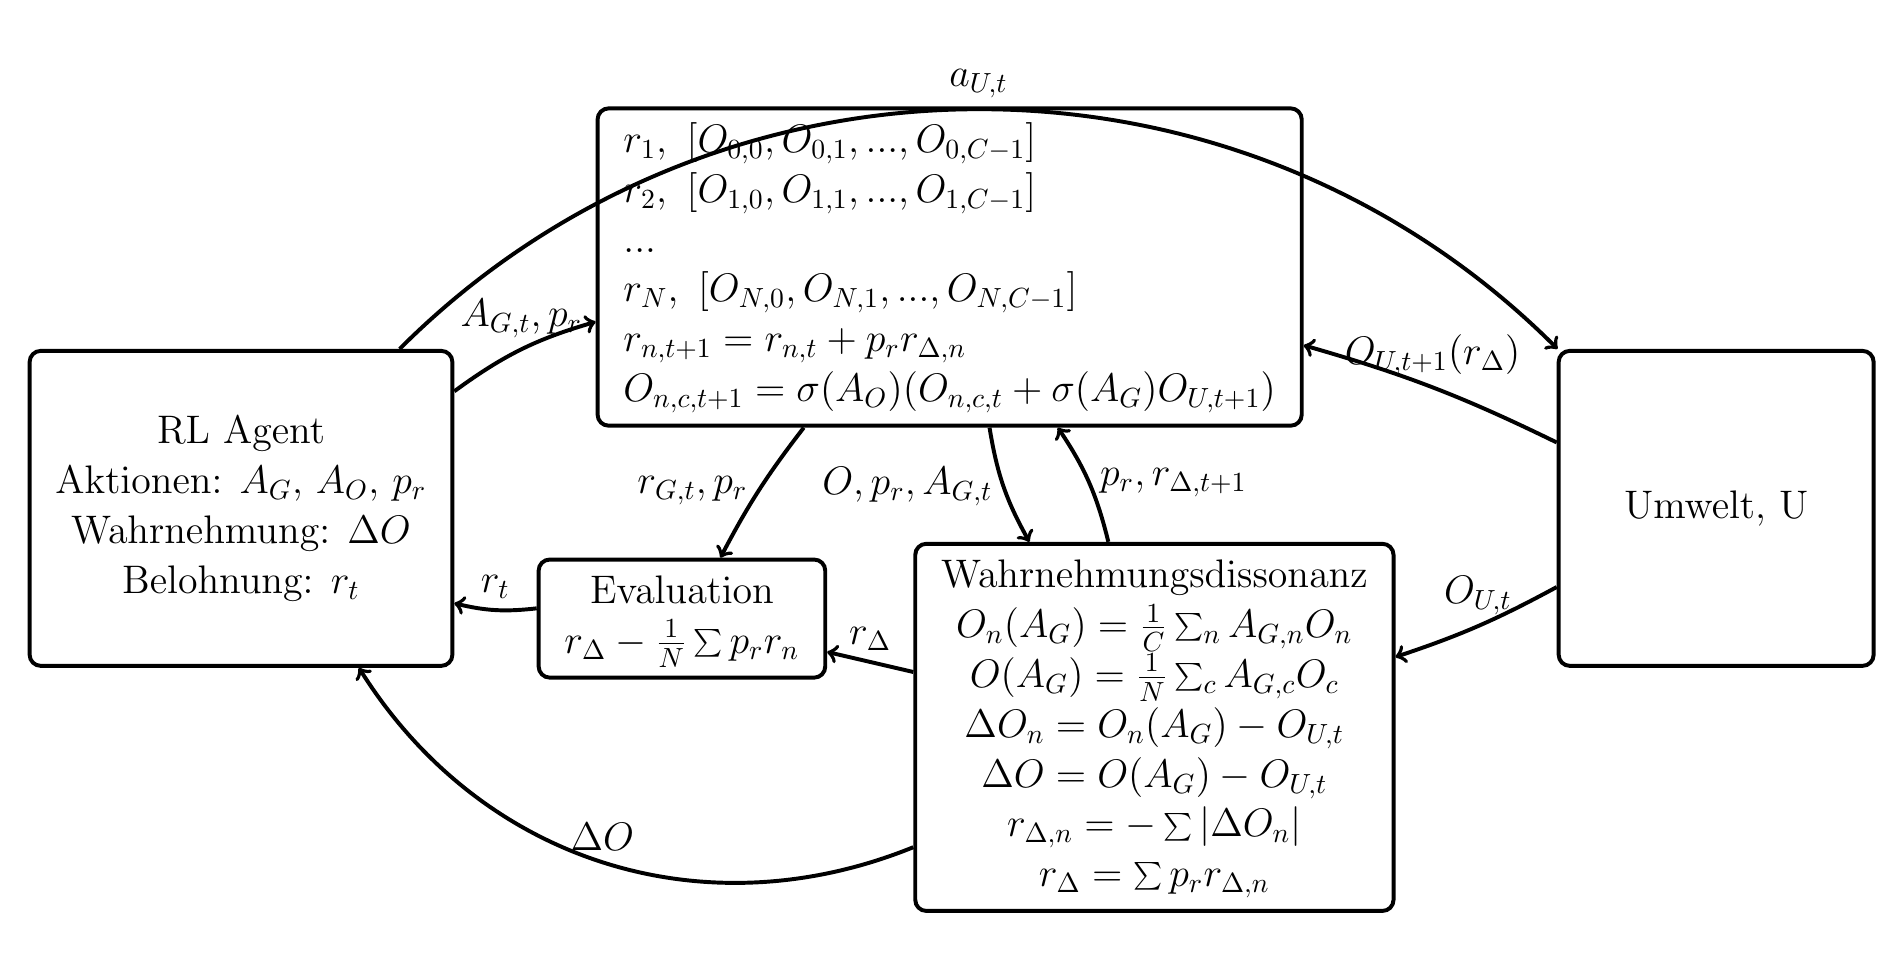
\begin{tikzpicture}[node distance=2cm, auto]
  % Nodes 
  \node (agent) [minimum width=4cm, minimum height=4cm, rounded corners] {
    \begin{tabular}{c}  
      RL Agent\\ 
      Aktionen: $A_G$, $A_O$, $p_r$ \\
      Wahrnehmung: $\Delta O$ \\
      Belohnung: $r_t$
    \end{tabular}
    };
  \node (memory) [above=-1cm of agent, xshift=9cm, minimum width=6cm, minimum height=2cm, rounded corners]  {
      \begin{tabular}{l}
        $r_1,\ [O_{0,0}, O_{0,1}, ..., O_{0,C-1}]$ \\
        $r_2,\ [O_{1,0}, O_{1,1}, ..., O_{1,C-1}]$ \\
        ... \\
        $r_{N},\ [O_{N,0}, O_{N,1}, ..., O_{N,C-1}]$  \\
      $ r_{n, t + 1} = r_{n, t} + p_r r_{\Delta, n} $ \\
      $ O_{n, c, t + 1} = \sigma(A_O)(O_{n, c, t} + \sigma{(A_{G})} O_{U, t + 1}) $ 
      \end{tabular}
  };
  \node (world) [right=14cm of agent, minimum width=4cm, minimum height=4cm, rounded corners] {Umwelt, U};
  \node (evaluator) [rectangle, below=-1.4cm of agent, xshift=5.6cm, rounded corners] {
    \begin{tabular}{c}  Evaluation \\ $r_{\Delta} - \frac{1}{N}\sum{ p_r r_n}$ \end{tabular}
  };
  \node (calculator) [rectangle, below=-1.6cm of agent, xshift=11.6cm, rounded corners] {
    \begin{tabular}{c} 
      Wahrnehmungsdissonanz \\ 
      $O_n(A_G) = \frac{1}{C} \sum_n A_{G, n} O_n$ \\ 
      $O(A_G) = \frac{1}{N} \sum_c A_{G, c} O_c$ \\ 
      $\Delta O_n = O_n(A_{G})-O_{U, t}$ \\ 
      $\Delta O = O(A_{G})-O_{U, t}$ \\ 
      $ r_{\Delta, n} = -\sum |\Delta O_{n}| $ \\
      $ r_{\Delta} = \sum p_r r_{\Delta, n} $
    \end{tabular}
  };

  \draw[->] (calculator) to[bend left=40] node[midway, above, draw=none, fill=none] {$\Delta O$} (agent);
  \draw[->] (memory) to[bend right=5] node[midway, left, draw=none, fill=none] {$r_{G, t}, p_r$} (evaluator);
  \draw[->] (world) to[bend left=5] node[midway, above, draw=none, fill=none] {$O_{U, t}$} (calculator);
  \draw[->] (memory) to[bend right=10] node[midway, left, draw=none, fill=none] {$O, p_r, A_{G, t}$} (calculator);
  \draw[->] (calculator) to[bend left=0] node[midway, above, draw=none, fill=none] {$r_{\Delta}$} (evaluator);
  \draw[->] (calculator) to[bend right=10] node[midway, right, draw=none, fill=none] {$p_r, r_{\Delta, t + 1}$} (memory);
  \draw[->] (agent) to[bend left=10] node[midway, above, draw=none, fill=none] {$A_{G, t}, p_r$} (memory);
  \draw[->] (agent) to[bend left=45] node[midway, above, draw=none, fill=none] {$a_{U, t}$} (world);
  \draw[->] (world) to[bend right=5] node[midway, above, draw=none, fill=none] {$O_{U, t+1}(r_{\Delta})$} (memory);
  \draw[->] (evaluator) to[bend left=10] node[midway, above, draw=none, fill=none] {$r_t$} (agent);
\end{tikzpicture}
\end{document}